\documentclass[conference]{IEEEtran}
\IEEEoverridecommandlockouts

\usepackage{amsmath,amssymb,amsfonts}
\usepackage{graphicx}
\usepackage{textcomp}
\usepackage{xcolor}
\usepackage[backend=biber,style=numeric]{biblatex}
\addbibresource{report.bib}

\graphicspath{{assets/latex/}}

\begin{document}

\title{CS6524 Computer Vision Lab. 1\\ Silhouettes and Fourier Epicycles}

\author{\IEEEauthorblockN{James Doherty}
\IEEEauthorblockA{\textit{Immersive Software Engineering} \\
\textit{University of Limerick}\\
23374039}}

\maketitle

\begin{abstract}
This lab extracts object silhouettes with linear spatial filters, orders the border into a closed trajectory, and rebuilds that shape with 1D Fourier descriptors. Six images were tested. Low harmonic counts give a rough outline and higher counts recover finer detail. Failures mostly come from broken borders after thresholding.
\end{abstract}

\section{Introduction}
The goal is to turn a normal photo into a closed 2D outline and then approximate that outline with rotating Fourier harmonics (epicycles). The input is a raw image, not a ready-made contour. I implement the filters myself with small convolution kernels and use \texttt{numpy.fft} for the descriptor stage~\cite{foundationsCVbook}.

\section{Method}
\subsection{Preprocessing}
Each image is converted to grayscale and smoothed with a Gaussian kernel. A fixed threshold then makes a binary mask. If the object is darker than the background I invert before thresholding. The border is taken as the binary mask minus its morphological erosion, which gives a thin silhouette. Kernel size, $\sigma$, threshold and invert flag are stored per image in a YAML file under \texttt{in/}.

\subsection{Trajectory}
Edge pixels are sorted by repeated nearest-neighbour walking, then resampled to a fixed arc-length length $N$ (usually 400). The ordered samples form a complex signal
\begin{equation}
z[n] = x[n] + i\, y[n].
\end{equation}

\subsection{Fourier reconstruction}
I compute $Z = \mathrm{FFT}(z)$, keep the strongest fraction of coefficients, zero the rest, and invert. The output mosaics show reconstructions from 5\% to 100\% of the dominant harmonics in steps of 5\%.

\section{Results and discussion}
On clean subjects with a simple background (for example the provided duck) the pipeline produces a usable closed path and the Fourier plots improve smoothly as more harmonics are kept. With only a few coefficients the shape is blob-like. Around 20 to 40\% the main proportions appear. Near 100\% the curve matches the extracted border closely.

The main failure mode is threshold choice. If the threshold is too aggressive the mask sprouts holes or loses thin parts, and the nearest-neighbour tracer then jumps across gaps, leaving chord-like shortcuts in the trajectory. Hand-tuned YAML values reduce this but do not remove it. A better next step would be adaptive thresholding or a connectivity cleanup before tracing.

Overall the lab shows that spatial filtering plus a 1D DFT is enough to encode a silhouette, and that reconstruction quality is directly controlled by how many harmonics are retained.

\begin{figure}[t]
\centerline{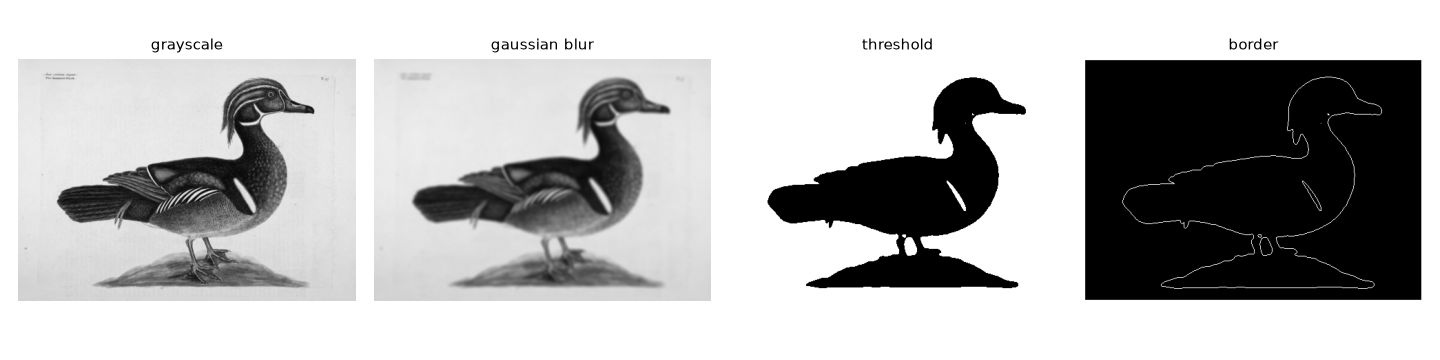
\includegraphics[width=\columnwidth]{fig1.png}}
\caption{Preprocessing for the duck image: grayscale, blur, threshold and border.}
\label{fig:transforms}
\end{figure}

\begin{figure}[t]
\centerline{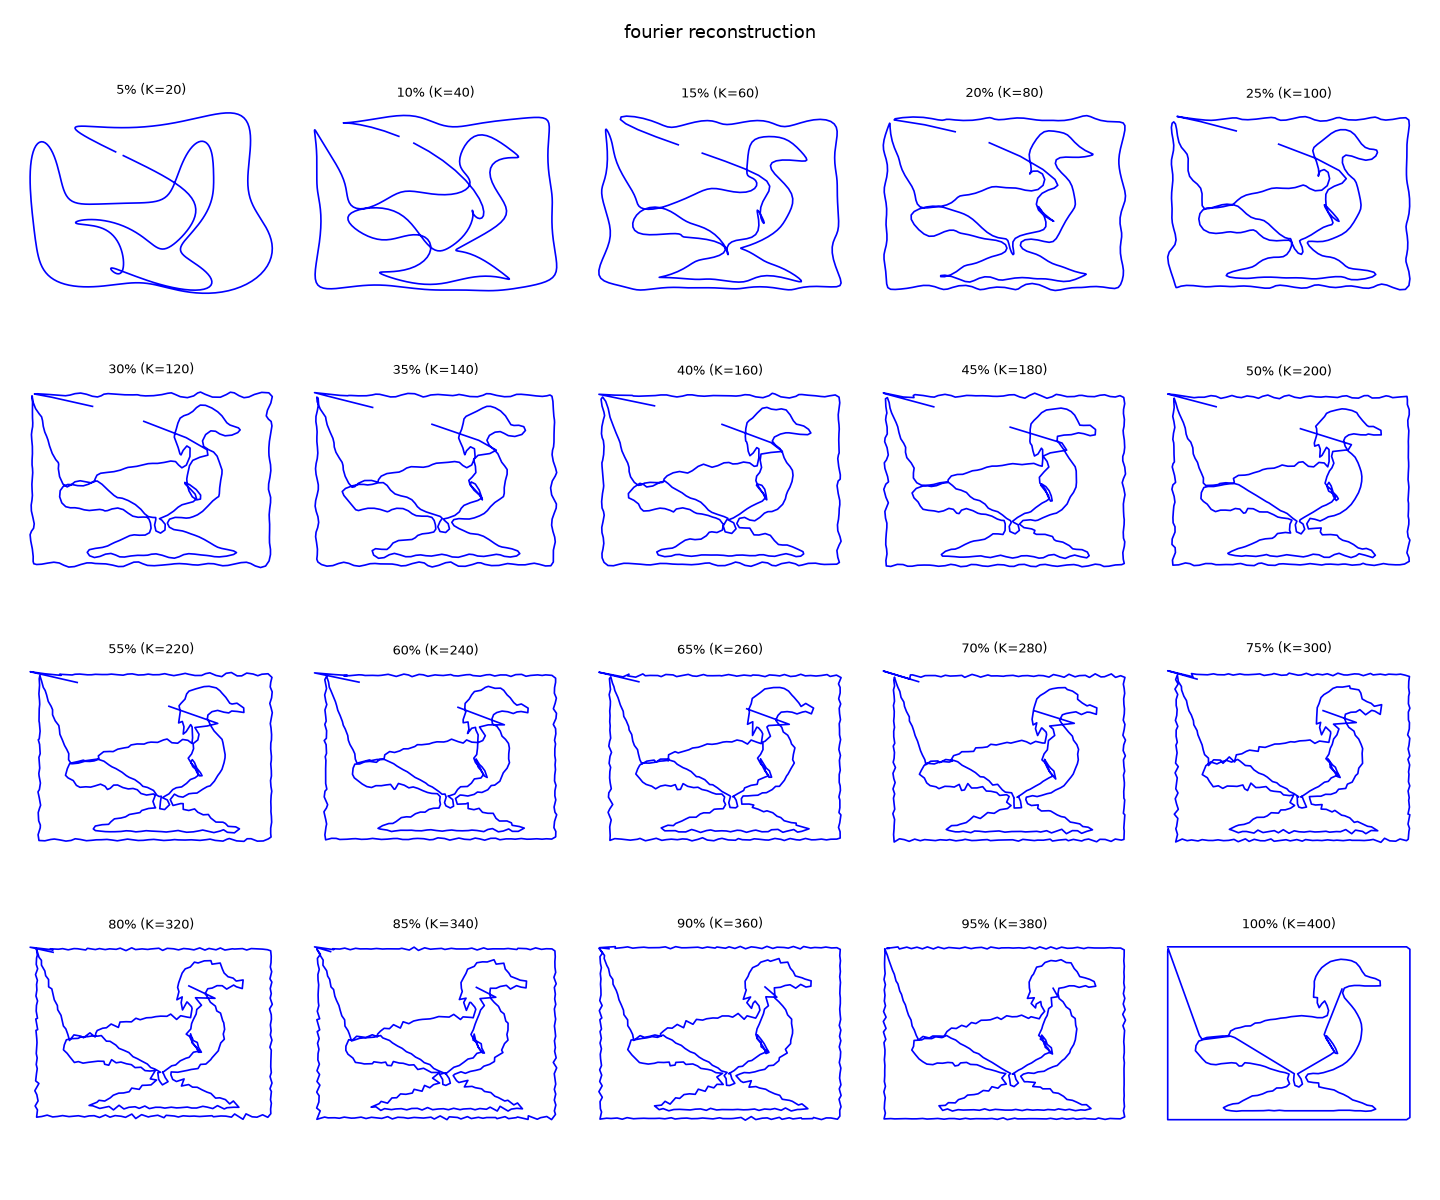
\includegraphics[width=\columnwidth]{fig2.png}}
\caption{Fourier reconstructions of the duck silhouette from 5\% to 100\% of the dominant harmonics.}
\label{fig:final}
\end{figure}

\printbibliography

\end{document}
